%\begin{enumerate}[label=\arabic*.,ref=\theenumi]
\begin{enumerate}[label=\thesection.\arabic*.,ref=\thesection.\theenumi]
\numberwithin{equation}{enumi}
%2.1.1
\item Consider the Magnitude Bode Plot and Phase Bode Plot \ref{fig:ee18btech11014_Bode} of Open-Loop Transfer Function of an Amplifier. Estimate the Open-Loop Transfer Function. (Assume $'A'$ as $'G'$ and $'\beta'$ as $'H'$)
\begin{figure}[ht!]
	\begin{center}
		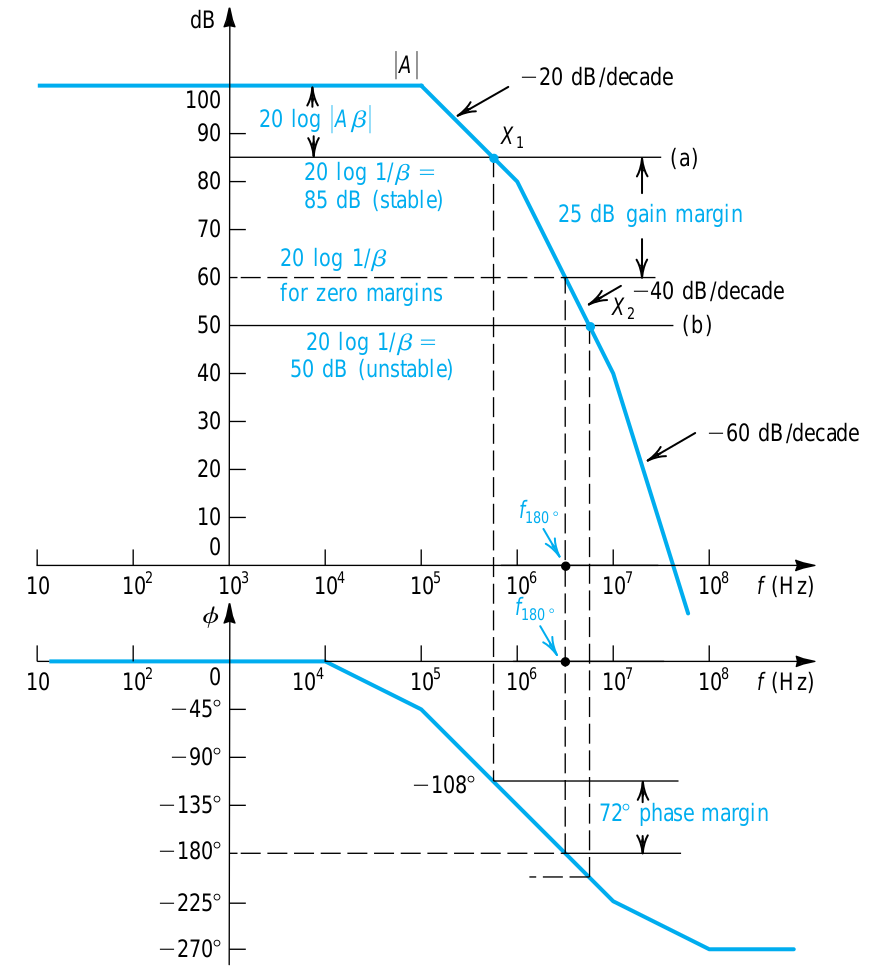
\includegraphics[width=\columnwidth]{./figs/ee18btech11014/ee18btech11014_figa.eps}
	\end{center}
	\caption{Magnitude and Phase Bode Plot}
	\label{fig:ee18btech11014_Bode}
\end{figure}\\
\solution Let $G(f)$ be the Open-Loop Transfer Function,
\begin{align}
\label{eq:ee18btech11014_G_piece}
G(f) = 
\begin{cases} 
      100 & 0 < f < 10^{5} \\
      200-20\log(f) & 10^{5} < f < 10^{6} \\
      320-40\log(f) & 10^{6} < f < 10^{7} \\
      460-60\log(f) & 10^{7} < f  \\
\end{cases}
\end{align}

\begin{align}
\nabla G(f) &= \dfrac{d(G(f))}{d(\log(f))} =
\begin{cases} 
        0 & 0 < f < 10^{5} \\
      -20 & 10^{5} < f < 10^{6} \\
      -40 & 10^{6} < f < 10^{7} \\
      -60 & 10^{7} < f  \\ 
\end{cases}
\end{align}

As we know that, \textbf{When a pole is encountered the slope always decreases by 20 dB/decade} and \textbf{When a zero is encountered the slope always increases by 20 dB/decade}. So, by observing Fig. \ref{fig:ee18btech11014_Bode} it can be concluded that we are having Poles at $f=10^{5} Hz, 10^{6} Hz, 10^{7} Hz$ and No Zeros.\\

So, the Open-Loop Transfer Function $G(f)$ is
\begin{align}
\label{eq:ee18btech11014_G}
	G(f) = \dfrac{10^{5}}{\left(1+j\frac{f}{10^{5}}\right)\left(1+j\frac{f}{10^{6}}\right)\left(1+j\frac{f}{10^{7}}\right)}
\end{align}\\
%-------------------------------------------------------------------------------------------------%
%2.1.2
\item Calculate the Phase of Open-Loop Transfer Function.\\
\solution
%
\begin{multline}
\label{eq:ee18btech11014_G_ang}
\phi\brak{f} =
\\
-\sbrak{\tan ^{-1}\brak{\frac{f}{10^{5}}}+\tan ^{-1}\brak{\frac{f}{10^{6}}}+\tan ^{-1}\brak{\frac{f}{10^{7}}}}
\end{multline}
%-------------------------------------------------------------------------------------------------%

\item Verify  \eqref{eq:ee18btech11014_G} by plotting the 
Magnitude and Phase Bode Plots of $G(f)$ and comparing with \eqref{eq:ee18btech11014_G_piece}
\\
\solution
See Fig.  \ref{fig:ee18btech11014_Bode Plot}
\begin{figure}[ht!]
	\begin{center}
		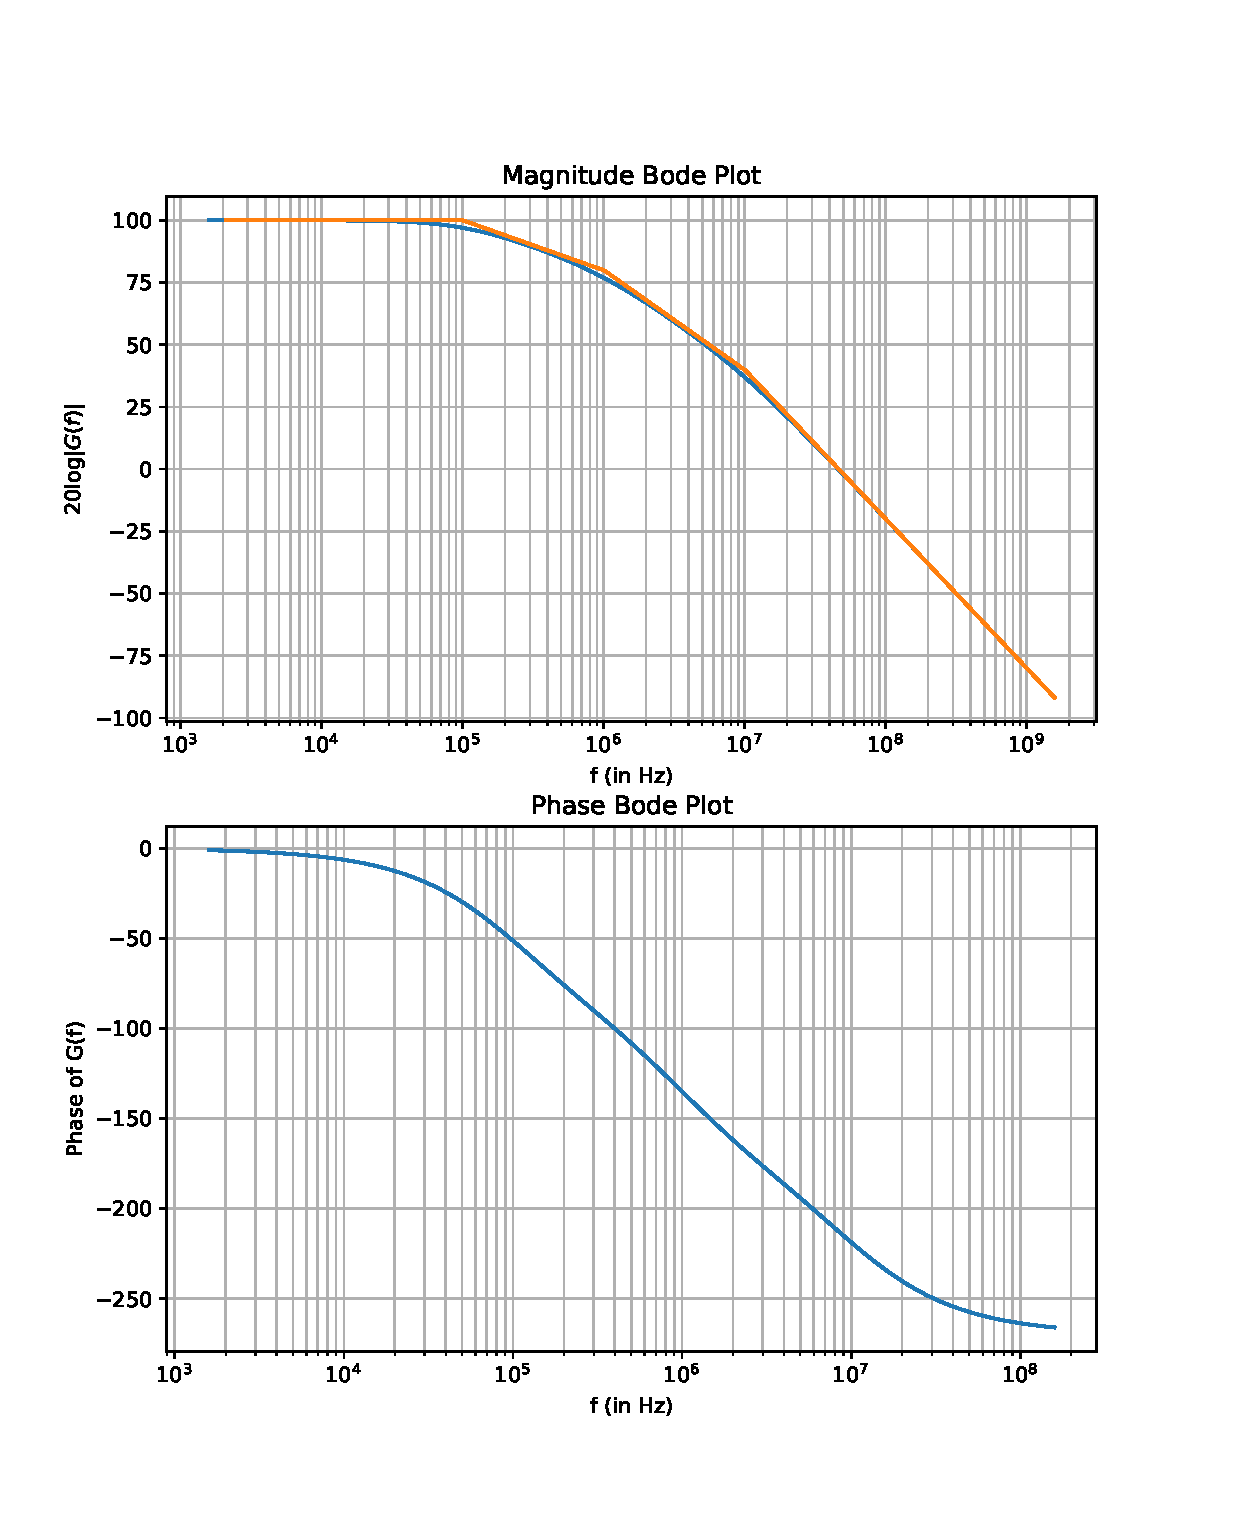
\includegraphics[width=\columnwidth]{./figs/ee18btech11014/Bode_Plot.eps}
	\end{center}
	\caption{Magnitude Bode Plot}
	\label{fig:ee18btech11014_Bode Plot}
\end{figure}

Python Code for Bode Plot is at
\begin{lstlisting}
codes/ee18btech11014/Bode_Plot.py
\end{lstlisting}

%-------------------------------------------------------------------------------------------------%
%2.1.3
\item Find the PM from  Fig. 	\ref{fig:ee18btech11014_Bode}, given that he feedback gain $H(f)$ is constant and given by 
\begin{align}
20 \log \brak{\frac{1}{H(f) }} &= 85 dB
\\
\text{or, } H(f) &= 5.623 \times 10^{-5}.
\label{eq:ee18btech11014_H}
\end{align}
\\
\solution From the figure, 
\begin{align}
\label{eq:ee18btech11014_G_f1}
20 \log \abs{G(f_1)} &= 85 dB
\\
\implies 20 \log \abs{G(f_1)} & = 20 \log \brak{\frac{1}{H(f_1) }}
\\
\text{or, } \abs{G(f_1)H(f_1)} &= 1
\end{align}
and 
\begin{align}
\label{eq:ee18btech11014_f1}
f_1 = 0.493 MHz, 
\end{align}
from \eqref{eq:ee18btech11014_G_f1} and \eqref{eq:ee18btech11014_G}.
Also,
%
\begin{align}
\because \phase{H(f)} &= 0, \forall f
\\
\phase{G(f_1)H(f_1)} &= \phase{G(f_1)} = -108 \degree
\\
\implies PM &= 180 \degree - 108 \degree = 72 \degree
\end{align}
using \eqref{eq:ee18btech11014_f1} in \eqref{eq:ee18btech11014_G_ang}.

%-------------------------------------------------------------------------------------------------%
\item Find the GM.
\\
\solution The crossover frequency $f_{\pi}$ is defined as 
\begin{align}
\phase{G\brak{f_{\pi}}H\brak{f_{\pi}}} &= 180 \degree
\\
\implies \phase{G\brak{f_{\pi}}} &= 180 \degree
\\
\implies f_{\pi} &= 3.34 MHz
\end{align}
by solving \eqref{eq:ee18btech11014_G_ang}.
From Fig. \ref{fig:ee18btech11014_Bode}, 
\begin{align}
%\label{eq:ee18btech11014_G_f1}
20 \log \abs{G(f_\pi)} &= 60 dB
\\
\implies 20 \log \abs{G(f_\pi)} &-  20 \log \brak{\frac{1}{H(f_\pi) }}   
\nonumber \\
&= \brak{60 -85} dB
\\
\implies GM &= \abs{20 \log \abs{G(f_\pi)H(f_\pi) }} 
\nonumber \\
&= 25 dB
\end{align}
%

%-------------------------------------------------------------------------------------------------%
%2.1.8
\item Break the Transfer Function $G(s)$ into Simple Blocks and create a block diagram.
\\
\solution From \eqref{eq:ee18btech11014_G}

\begin{align}
\label{eq:ee18btech11014_Gs}
	G(s) = \dfrac{10^{5}}{\left(1+\frac{s}{2\pi10^{5}}\right)\left(1+\frac{s}{2\pi10^{6}}\right)\left(1+\frac{s}{2\pi10^{7}}\right)}
\end{align}
%
The block diagram is available in 
Fig. 	\ref{fig:ee18btech11014_RC Circuit_block}
%
\begin{figure}[ht!]
	\begin{center}
		\resizebox{\columnwidth}{!}{\tikzstyle{block} = [draw, rectangle, 
    minimum height=2em, minimum width=4em]
\tikzstyle{sum} = [draw, circle, node distance=1cm]
\tikzstyle{input} = [coordinate]
\tikzstyle{output} = [coordinate]
\tikzstyle{pinstyle} = [pin edge={to-,thin,black}]

% The block diagram code is probably more verbose than necessary
\begin{tikzpicture}[auto, node distance=3cm,>=latex']
    % We start by placing the blocks
    \node [input, name=input] {};
    \node [block, right of=input] (p1) {$\frac{1}{1+\frac{s}{2\pi \times 10^{5}}}$};
    \node [block, right of=p1] (p2) {$\frac{1}{1+\frac{s}{2\pi \times 10^{6}}}$};
    \node [block, right of=p2] (p3) {$\frac{1}{1+\frac{s}{2\pi \times 10^{7}}}$};
    \node [block, right of=p3] (g) {$10^{5}$};
    \node [output, right of=g] (output) {};

    % Once the nodes are placed, connecting them is easy. 
    \draw [draw,->] (input) -- node {$v_{s}$} (p1);
    \draw [->] (p1) -- node {$v_{a}$} (p2);
    \draw [->] (p2) -- node {$v_{b}$} (p3);
    \draw [->] (p3) -- node {$v_{c}$} (g);
    \draw [->] (g) -- node {$v_{o}$} (output);
\end{tikzpicture}
}
	\end{center}
	\caption{}
	\label{fig:ee18btech11014_RC Circuit_block}
\end{figure}

%-------------------------------------------------------------------------------------------------%
%2.1.9
\item Find the Gain of RC-Circuit in Fig. \ref{fig:ee18btech11014_RC Circuit} and identify the pole location.
\begin{figure}[ht!]
	\begin{center}
		\resizebox{\columnwidth/2}{!}{\begin{circuitikz}[american]
\tikzset{quad/.style={draw, minimum height=2.4cm, minimum width=4cm}}
\node[quad] (A) at (0,0) {$H$};
\draw ($(A.north west)!.175!(A.west)$) to[short,-o] ++(-2,0) -- (-5,1)
      ($(A.south west)!.175!(A.west)$) to[short,-o] ++(-2,0) -- (-5,-1)
      ($(A.north east)!.175!(A.east)$) to[short,-o] ++(1,0)
      ($(A.south east)!.175!(A.east)$) to[short,-o] ++(1,0);

\draw (-5,-1) to[short, i=$I_{f}$] (-5,1);
\draw (-5,-1) to[closing switch, o-o] (-5,-2) node[ground](GND){};

\draw (3,-1) -- (5,-1) to[isource, l= $I_{o}$] (5,1) -- (3,1);

\end{circuitikz}
}
	\end{center}
	\caption{}
	\label{fig:ee18btech11014_RC Circuit}
\end{figure}

\solution
\begin{align}
v_o &= v_i \frac{\frac{1}{sc}}{R + \frac{1}{sC}}
\\
\implies \frac{v_o}{v_i}&= \frac{1}{1+sCR}
\label{eqLee18btech11014_RC}
%I = \frac{v_{input}}{R + \frac{1}{Cs}}\\
%v_{output} = I \times \frac{1}{Cs}\\
%v_{output} = \frac{v_{input} \times \frac{1}{Cs}}{R + \frac{1}{Cs}}\\
%\frac{v_{output}}{v_{input}} = \frac{1}{RCs + 1}\\
%s = j2\pi f\\
%Gain = \frac{v_{output}}{v_{input}} = \frac{1}{j2\pi RCf + 1}
\end{align}
%
Thus, there is a pole at
%
\begin{align}
s = -\frac{1}{RC}
\end{align}
%
%-------------------------------------------------------------------------------------------------%
%
%2.1.11
\item Design a circuit for $G(s)$.
\\
\solution \eqref{eq:ee18btech11014_Gs} can be expressed as
%
\begin{align}
\because G(s) = \frac{G_0}{\brak{1+sC_1R_1}\brak{1+sC_2R_2}\brak{1+sC_3R_3}}
\end{align}
%
where the parameters are available in Table \ref{table:ee18btech11014_table1}.  Choosing an OPAMP of gain %
$G_0$ and noting from \eqref{eqLee18btech11014_RC} that each of the blocks in Fig. 	\ref{fig:ee18btech11014_RC Circuit_block} can be realised through the RC circuit in Fig. 	\ref{fig:ee18btech11014_RC Circuit} with parameters in Table \ref{table:ee18btech11014_table1}, the circuit design is available in 
Fig. 	\ref{fig:ee18btech11014_Open-Loop Circuit}. 
%
\begin{table}[!ht]
\centering
%%%%%%%%%%%%%%%%%%%%%%%%%%%%%%%%%%%%%%%%%%%%%%%%%%%%%%%%%%%%%%%%%%%%%%
%%                                                                  %%
%%  This is the header of a LaTeX2e file exported from Gnumeric.    %%
%%                                                                  %%
%%  This file can be compiled as it stands or included in another   %%
%%  LaTeX document. The table is based on the longtable package so  %%
%%  the longtable options (headers, footers...) can be set in the   %%
%%  preamble section below (see PRAMBLE).                           %%
%%                                                                  %%
%%  To include the file in another, the following two lines must be %%
%%  in the including file:                                          %%
%%        \def\inputGnumericTable{}                                 %%
%%  at the beginning of the file and:                               %%
%%        \input{name-of-this-file.tex}                             %%
%%  where the table is to be placed. Note also that the including   %%
%%  file must use the following packages for the table to be        %%
%%  rendered correctly:                                             %%
%%    \usepackage[latin1]{inputenc}                                 %%
%%    \usepackage{color}                                            %%
%%    \usepackage{array}                                            %%
%%    \usepackage{longtable}                                        %%
%%    \usepackage{calc}                                             %%
%%    \usepackage{multirow}                                         %%
%%    \usepackage{hhline}                                           %%
%%    \usepackage{ifthen}                                           %%
%%  optionally (for landscape tables embedded in another document): %%
%%    \usepackage{lscape}                                           %%
%%                                                                  %%
%%%%%%%%%%%%%%%%%%%%%%%%%%%%%%%%%%%%%%%%%%%%%%%%%%%%%%%%%%%%%%%%%%%%%%



%%  This section checks if we are begin input into another file or  %%
%%  the file will be compiled alone. First use a macro taken from   %%
%%  the TeXbook ex 7.7 (suggestion of Han-Wen Nienhuys).            %%
\def\ifundefined#1{\expandafter\ifx\csname#1\endcsname\relax}


%%  Check for the \def token for inputed files. If it is not        %%
%%  defined, the file will be processed as a standalone and the     %%
%%  preamble will be used.                                          %%
\ifundefined{inputGnumericTable}

%%  We must be able to close or not the document at the end.        %%
	\def\gnumericTableEnd{\end{document}}


%%%%%%%%%%%%%%%%%%%%%%%%%%%%%%%%%%%%%%%%%%%%%%%%%%%%%%%%%%%%%%%%%%%%%%
%%                                                                  %%
%%  This is the PREAMBLE. Change these values to get the right      %%
%%  paper size and other niceties.                                  %%
%%                                                                  %%
%%%%%%%%%%%%%%%%%%%%%%%%%%%%%%%%%%%%%%%%%%%%%%%%%%%%%%%%%%%%%%%%%%%%%%

	\documentclass[12pt%
			  %,landscape%
                    ]{report}
       \usepackage[latin1]{inputenc}
       \usepackage{fullpage}
       \usepackage{color}
       \usepackage{array}
       \usepackage{longtable}
       \usepackage{calc}
       \usepackage{multirow}
       \usepackage{hhline}
       \usepackage{ifthen}

	\begin{document}


%%  End of the preamble for the standalone. The next section is for %%
%%  documents which are included into other LaTeX2e files.          %%
\else

%%  We are not a stand alone document. For a regular table, we will %%
%%  have no preamble and only define the closing to mean nothing.   %%
    \def\gnumericTableEnd{}

%%  If we want landscape mode in an embedded document, comment out  %%
%%  the line above and uncomment the two below. The table will      %%
%%  begin on a new page and run in landscape mode.                  %%
%       \def\gnumericTableEnd{\end{landscape}}
%       \begin{landscape}


%%  End of the else clause for this file being \input.              %%
\fi

%%%%%%%%%%%%%%%%%%%%%%%%%%%%%%%%%%%%%%%%%%%%%%%%%%%%%%%%%%%%%%%%%%%%%%
%%                                                                  %%
%%  The rest is the gnumeric table, except for the closing          %%
%%  statement. Changes below will alter the table's appearance.     %%
%%                                                                  %%
%%%%%%%%%%%%%%%%%%%%%%%%%%%%%%%%%%%%%%%%%%%%%%%%%%%%%%%%%%%%%%%%%%%%%%

\providecommand{\gnumericmathit}[1]{#1} 
%%  Uncomment the next line if you would like your numbers to be in %%
%%  italics if they are italizised in the gnumeric table.           %%
%\renewcommand{\gnumericmathit}[1]{\mathit{#1}}
\providecommand{\gnumericPB}[1]%
{\let\gnumericTemp=\\#1\let\\=\gnumericTemp\hspace{0pt}}
 \ifundefined{gnumericTableWidthDefined}
        \newlength{\gnumericTableWidth}
        \newlength{\gnumericTableWidthComplete}
        \newlength{\gnumericMultiRowLength}
        \global\def\gnumericTableWidthDefined{}
 \fi
%% The following setting protects this code from babel shorthands.  %%
 \ifthenelse{\isundefined{\languageshorthands}}{}{\languageshorthands{english}}
%%  The default table format retains the relative column widths of  %%
%%  gnumeric. They can easily be changed to c, r or l. In that case %%
%%  you may want to comment out the next line and uncomment the one %%
%%  thereafter                                                      %%
\providecommand\gnumbox{\makebox[0pt]}
%%\providecommand\gnumbox[1][]{\makebox}

%% to adjust positions in multirow situations                       %%
\setlength{\bigstrutjot}{\jot}
\setlength{\extrarowheight}{\doublerulesep}

%%  The \setlongtables command keeps column widths the same across  %%
%%  pages. Simply comment out next line for varying column widths.  %%
\setlongtables

\setlength\gnumericTableWidth{%
	75pt+%
	75pt+%
0pt}
\def\gumericNumCols{2}
\setlength\gnumericTableWidthComplete{\gnumericTableWidth+%
         \tabcolsep*\gumericNumCols*2+\arrayrulewidth*\gumericNumCols}
\ifthenelse{\lengthtest{\gnumericTableWidthComplete > \linewidth}}%
         {\def\gnumericScale{\ratio{\linewidth-%
                        \tabcolsep*\gumericNumCols*2-%
                        \arrayrulewidth*\gumericNumCols}%
{\gnumericTableWidth}}}%
{\def\gnumericScale{1}}

%%%%%%%%%%%%%%%%%%%%%%%%%%%%%%%%%%%%%%%%%%%%%%%%%%%%%%%%%%%%%%%%%%%%%%
%%                                                                  %%
%% The following are the widths of the various columns. We are      %%
%% defining them here because then they are easier to change.       %%
%% Depending on the cell formats we may use them more than once.    %%
%%                                                                  %%
%%%%%%%%%%%%%%%%%%%%%%%%%%%%%%%%%%%%%%%%%%%%%%%%%%%%%%%%%%%%%%%%%%%%%%

\ifthenelse{\isundefined{\gnumericColA}}{\newlength{\gnumericColA}}{}\settowidth{\gnumericColA}{\begin{tabular}{@{}p{75pt*\gnumericScale}@{}}x\end{tabular}}
\ifthenelse{\isundefined{\gnumericColB}}{\newlength{\gnumericColB}}{}\settowidth{\gnumericColB}{\begin{tabular}{@{}p{75pt*\gnumericScale}@{}}x\end{tabular}}

\begin{tabular}[c]{%
	b{\gnumericColA}%
	b{\gnumericColB}%
	}

%%%%%%%%%%%%%%%%%%%%%%%%%%%%%%%%%%%%%%%%%%%%%%%%%%%%%%%%%%%%%%%%%%%%%%
%%  The longtable options. (Caption, headers... see Goosens, p.124) %%
%	\caption{The Table Caption.}             \\	%
% \hline	% Across the top of the table.
%%  The rest of these options are table rows which are placed on    %%
%%  the first, last or every page. Use \multicolumn if you want.    %%

%%  Header for the first page.                                      %%
%	\multicolumn{3}{c}{The First Header} \\ \hline 
%	\multicolumn{1}{c}{colTag}	%Column 1
%	&\multicolumn{1}{c}{colTag}	%Column 2
%	&\multicolumn{1}{c}{colTag}	\\ \hline %Last column
%	\endfirsthead

%%  The running header definition.                                  %%
%	\hline
%	\multicolumn{3}{l}{\ldots\small\slshape continued} \\ \hline
%	\multicolumn{1}{c}{colTag}	%Column 1
%	&\multicolumn{1}{c}{colTag}	%Column 2
%	&\multicolumn{1}{c}{colTag}	\\ \hline %Last column
%	\endhead

%%  The running footer definition.                                  %%
%	\hline
%	\multicolumn{3}{r}{\small\slshape continued\ldots} \\
%	\endfoot

%%  The ending footer definition.                                   %%
%	\multicolumn{3}{c}{That's all folks} \\ \hline 
%	\endlastfoot
%%%%%%%%%%%%%%%%%%%%%%%%%%%%%%%%%%%%%%%%%%%%%%%%%%%%%%%%%%%%%%%%%%%%%%

\hhline{|-|-}
	 \multicolumn{1}{|p{\gnumericColA}|}%
	{\gnumericPB{\centering}Circuit Element}
	&\multicolumn{1}{p{\gnumericColB}|}%
	{\gnumericPB{\centering}Value}
	
\\
\hhline{|--|}
	 \multicolumn{1}{|p{\gnumericColA}|}%
	{\gnumericPB{\centering}$R_{1}$}
	&\multicolumn{1}{p{\gnumericColB}|}%
	{\gnumericPB{\centering}$10^2\ohm$}

\\
\hhline{|--|}
	 \multicolumn{1}{|p{\gnumericColA}|}%
	{\gnumericPB{\centering}$R_{2}$}
	&\multicolumn{1}{p{\gnumericColB}|}%
	{\gnumericPB{\centering}$10^3\ohm$}

\\
\hhline{|--|}
	 \multicolumn{1}{|p{\gnumericColA}|}%
	{\gnumericPB{\centering}$R_{3}$}
	&\multicolumn{1}{p{\gnumericColB}|}%
	{\gnumericPB{\centering}$10^4\ohm$}

\\
\hhline{|--|}
	 \multicolumn{1}{|p{\gnumericColA}|}%
	{\gnumericPB{\centering}$C_{1}$}
	&\multicolumn{1}{p{\gnumericColB}|}%
	{\gnumericPB{\centering}$\frac{10^{-9}}{2\pi}F$}

\\
\hhline{|--|}
	 \multicolumn{1}{|p{\gnumericColA}|}%
	{\gnumericPB{\centering}$C_{2}$}
	&\multicolumn{1}{p{\gnumericColB}|}%
	{\gnumericPB{\centering}$\frac{10^{-9}}{2\pi}F$}

\\
\hhline{|--|}
	 \multicolumn{1}{|p{\gnumericColA}|}%
	{\gnumericPB{\centering}$C_{3}$}
	&\multicolumn{1}{p{\gnumericColB}|}%
	{\gnumericPB{\centering}$\frac{10^{-9}}{2\pi}F$}
\\
\hhline{|-|-}
\end{tabular}

\ifthenelse{\isundefined{\languageshorthands}}{}{\languageshorthands{\languagename}}
\gnumericTableEnd

\caption{}
\label{table:ee18btech11014_table1}
\end{table}
%
\begin{figure}[ht!]
	\begin{center}
		\resizebox{\columnwidth/1}{!}{\begin{circuitikz}[american]

\draw (2,2)  node[op amp] (OA) {};
\draw (OA.up) -- ++(0, 0.3) node[vcc]{$+10V$};
\draw (OA.down) -- ++(0,-0.3) node[vee]{$-10V$};
\draw (OA.+) -- (0,1.5) to[vsourcesin, l= $v_{s}$] (0,0) node[ground](GND){};
\draw (OA.-) -- (0,2.5) node[ground, rotate=270](GND){};
\draw (OA.out) -- (3,2) node[label={above:$v_{a}$}]{};
\draw (3,2) to[R=$R_{1}$] (5.5,2) node[label={above:$v_{b}$}]{} to[C,l_=$C_{1}$] (5.5,0) node[ground](GND){};

\draw (7.5,2.5) node[op amp] (OB) {};
\draw (OB.up) -- ++(0, 0.3) node[vcc]{$+10V$};
\draw (OB.down) -- ++(0,-0.3) node[vee]{$-10V$};
\draw (OB.+) -- (5.5,2);
\draw (OB.-) -- ++(-0.5,0) node[ground,rotate=270](GND){};;
\draw (OB.out) to[R=$R_{2}$] (10.5,2.5) node[label={above:$v_{c}$}]{} to[C,l_=$C_{2}$] (10.5,0) node[ground](GND){};

\draw (12.5,3) node[op amp] (OC) {};
\draw (OC.up) -- ++(0, 0.3) node[vcc]{$+10V$};
\draw (OC.down) -- ++(0,-0.3) node[vee]{$-10V$};
\draw (OC.+) -- (10.5,2.5);
\draw (OC.-) -- ++(-0.5,0) node[ground,rotate=270](GND){};;
\draw (OC.out) to[R=$R_{3}$] (15.5,3) node[label={right:$v_{o}$}]{} to[C,l_=$C_{3}$] (15.5,0) node[ground](GND){};

\end{circuitikz}
}
	\end{center}
	\caption{}
	\label{fig:ee18btech11014_Open-Loop Circuit}
\end{figure}
 
%Assuming, Open-Loop Gain of Operational Amplifier is $10^{5}$ and also assuming Operational Amplifier doesnt have any Poles.\\
%Equivalent Circuit of the circuit is
%\begin{figure}[ht!]
%	\begin{center}
%		\resizebox{\columnwidth/1}{!}{\begin{circuitikz}[american]

\draw (0,0) node[ground](GND){} to[vsourcesin, l= $v_{s}$] (0,2) to[short,-o] (1,2) node[label={below:$+$}]{};
\draw (1,0) node[ground](GND){} to[short,-o] (1,0.1) node[label={above:$-$}] {};
\draw (3,2) node[label={above:$v_{a}$}]{};
\draw (1,0.625) node[label={$v_{i}$}] {};
\draw (3,0) node[ground](GND){} to[vsourcesin, l= $10^5 v_{i}$] (3,2);
\draw (3,2) to[R=$10^{2}\ohm$] (5.5,2) node[label={above:$v_{b}$}]{} to[C,l_=$\frac{10^{-9}}{2\pi}F$] (5.5,0) node[ground](GND){};
\draw (5.5,2) to[R=$10^{3}\ohm$] (8,2) node[label={above:$v_{c}$}]{} to[C,l_=$\frac{10^{-9}}{2\pi}F$] (8,0) node[ground](GND){};
\draw (8,2) to[R=$10^{4}\ohm$] (10.5,2) to[C,l_=$\frac{10^{-9}}{2\pi}F$] (10.5,0) node[ground](GND){};
\draw (10.5,2) -- (11.5,2) node[label={above:$v_{o}$}]{};

\end{circuitikz}
}
%	\end{center}
%	\caption{}
%	\label{fig:ee18btech11014_Equivalent Open-Loop Circuit}
%\end{figure}
%
%The cascade of RC Circuits are used to introduce poles in the circuit and Op-Amp are used to achieve the Gain required.\\
%
%At the Operational Amplifier,
%\begin{align}
%v_{i} = v_{s}\\
%v_{a} = 10^5 v_{i}\\
%v_{a} = 10^5 v_{s}
%\end{align}
%
%At the first RC-Circuit,
%\begin{align}
%p_{1} = \frac{1}{R_{1}C_{1}}\\
%v_{b} = \frac{v_{a}}{1 + \frac{s}{p_{1}}}\\
%v_{b} = \frac{10^5 v_{i}}{1 + \frac{s}{p_{1}}}
%\end{align}
%
%At the second RC-Circuit,
%\begin{align}
%p_{2} = \frac{1}{R_{2}C_{2}}\\
%v_{c} = \frac{v_{b}}{1 + \frac{s}{p_{2}}}\\
%v_{c} = \frac{10^5 v_{i}}{(1 + \frac{s}{p_{1}})(1 + \frac{s}{p_{2}})}
%\end{align}
%
%At the third RC-Circuit,
%\begin{align}
%p_{3} = \frac{1}{R_{3}C_{3}}\\
%v_{o} = \frac{v_{c}}{1 + \frac{s}{p_{3}}}
%\end{align}
%\begin{align}
%v_{o} = \frac{10^5 v_{i}}{(1 + \frac{s}{p_{1}})(1 + \frac{s}{p_{2}})(1 + \frac{s}{p_{3}})}
%\end{align}
%
%The RC Circuits should introduce poles at $f=10^{7} Hz, 10^{6} Hz, 10^{5} Hz$ respectively from left to right.\\
%Assuming the following values of circuit elements,\\
%
%Frequency can be calculated as
%\begin{align}
%f = \frac{1}{2\pi RC}
%\end{align}
%\begin{table}[!ht]
%\centering
%%%%%%%%%%%%%%%%%%%%%%%%%%%%%%%%%%%%%%%%%%%%%%%%%%%%%%%%%%%%%%%%%%%%%%%
%%                                                                  %%
%%  This is the header of a LaTeX2e file exported from Gnumeric.    %%
%%                                                                  %%
%%  This file can be compiled as it stands or included in another   %%
%%  LaTeX document. The table is based on the longtable package so  %%
%%  the longtable options (headers, footers...) can be set in the   %%
%%  preamble section below (see PRAMBLE).                           %%
%%                                                                  %%
%%  To include the file in another, the following two lines must be %%
%%  in the including file:                                          %%
%%        \def\inputGnumericTable{}                                 %%
%%  at the beginning of the file and:                               %%
%%        \input{name-of-this-file.tex}                             %%
%%  where the table is to be placed. Note also that the including   %%
%%  file must use the following packages for the table to be        %%
%%  rendered correctly:                                             %%
%%    \usepackage[latin1]{inputenc}                                 %%
%%    \usepackage{color}                                            %%
%%    \usepackage{array}                                            %%
%%    \usepackage{longtable}                                        %%
%%    \usepackage{calc}                                             %%
%%    \usepackage{multirow}                                         %%
%%    \usepackage{hhline}                                           %%
%%    \usepackage{ifthen}                                           %%
%%  optionally (for landscape tables embedded in another document): %%
%%    \usepackage{lscape}                                           %%
%%                                                                  %%
%%%%%%%%%%%%%%%%%%%%%%%%%%%%%%%%%%%%%%%%%%%%%%%%%%%%%%%%%%%%%%%%%%%%%%



%%  This section checks if we are begin input into another file or  %%
%%  the file will be compiled alone. First use a macro taken from   %%
%%  the TeXbook ex 7.7 (suggestion of Han-Wen Nienhuys).            %%
\def\ifundefined#1{\expandafter\ifx\csname#1\endcsname\relax}


%%  Check for the \def token for inputed files. If it is not        %%
%%  defined, the file will be processed as a standalone and the     %%
%%  preamble will be used.                                          %%
\ifundefined{inputGnumericTable}

%%  We must be able to close or not the document at the end.        %%
	\def\gnumericTableEnd{\end{document}}


%%%%%%%%%%%%%%%%%%%%%%%%%%%%%%%%%%%%%%%%%%%%%%%%%%%%%%%%%%%%%%%%%%%%%%
%%                                                                  %%
%%  This is the PREAMBLE. Change these values to get the right      %%
%%  paper size and other niceties.                                  %%
%%                                                                  %%
%%%%%%%%%%%%%%%%%%%%%%%%%%%%%%%%%%%%%%%%%%%%%%%%%%%%%%%%%%%%%%%%%%%%%%

	\documentclass[12pt%
			  %,landscape%
                    ]{report}
       \usepackage[latin1]{inputenc}
       \usepackage{fullpage}
       \usepackage{color}
       \usepackage{array}
       \usepackage{longtable}
       \usepackage{calc}
       \usepackage{multirow}
       \usepackage{hhline}
       \usepackage{ifthen}

	\begin{document}


%%  End of the preamble for the standalone. The next section is for %%
%%  documents which are included into other LaTeX2e files.          %%
\else

%%  We are not a stand alone document. For a regular table, we will %%
%%  have no preamble and only define the closing to mean nothing.   %%
    \def\gnumericTableEnd{}

%%  If we want landscape mode in an embedded document, comment out  %%
%%  the line above and uncomment the two below. The table will      %%
%%  begin on a new page and run in landscape mode.                  %%
%       \def\gnumericTableEnd{\end{landscape}}
%       \begin{landscape}


%%  End of the else clause for this file being \input.              %%
\fi

%%%%%%%%%%%%%%%%%%%%%%%%%%%%%%%%%%%%%%%%%%%%%%%%%%%%%%%%%%%%%%%%%%%%%%
%%                                                                  %%
%%  The rest is the gnumeric table, except for the closing          %%
%%  statement. Changes below will alter the table's appearance.     %%
%%                                                                  %%
%%%%%%%%%%%%%%%%%%%%%%%%%%%%%%%%%%%%%%%%%%%%%%%%%%%%%%%%%%%%%%%%%%%%%%

\providecommand{\gnumericmathit}[1]{#1} 
%%  Uncomment the next line if you would like your numbers to be in %%
%%  italics if they are italizised in the gnumeric table.           %%
%\renewcommand{\gnumericmathit}[1]{\mathit{#1}}
\providecommand{\gnumericPB}[1]%
{\let\gnumericTemp=\\#1\let\\=\gnumericTemp\hspace{0pt}}
 \ifundefined{gnumericTableWidthDefined}
        \newlength{\gnumericTableWidth}
        \newlength{\gnumericTableWidthComplete}
        \newlength{\gnumericMultiRowLength}
        \global\def\gnumericTableWidthDefined{}
 \fi
%% The following setting protects this code from babel shorthands.  %%
 \ifthenelse{\isundefined{\languageshorthands}}{}{\languageshorthands{english}}
%%  The default table format retains the relative column widths of  %%
%%  gnumeric. They can easily be changed to c, r or l. In that case %%
%%  you may want to comment out the next line and uncomment the one %%
%%  thereafter                                                      %%
\providecommand\gnumbox{\makebox[0pt]}
%%\providecommand\gnumbox[1][]{\makebox}

%% to adjust positions in multirow situations                       %%
\setlength{\bigstrutjot}{\jot}
\setlength{\extrarowheight}{\doublerulesep}

%%  The \setlongtables command keeps column widths the same across  %%
%%  pages. Simply comment out next line for varying column widths.  %%
\setlongtables

\setlength\gnumericTableWidth{%
	25pt+%
	50pt+%
	75pt+%
0pt}
\def\gumericNumCols{3}
\setlength\gnumericTableWidthComplete{\gnumericTableWidth+%
         \tabcolsep*\gumericNumCols*2+\arrayrulewidth*\gumericNumCols}
\ifthenelse{\lengthtest{\gnumericTableWidthComplete > \linewidth}}%
         {\def\gnumericScale{\ratio{\linewidth-%
                        \tabcolsep*\gumericNumCols*2-%
                        \arrayrulewidth*\gumericNumCols}%
{\gnumericTableWidth}}}%
{\def\gnumericScale{1}}

%%%%%%%%%%%%%%%%%%%%%%%%%%%%%%%%%%%%%%%%%%%%%%%%%%%%%%%%%%%%%%%%%%%%%%
%%                                                                  %%
%% The following are the widths of the various columns. We are      %%
%% defining them here because then they are easier to change.       %%
%% Depending on the cell formats we may use them more than once.    %%
%%                                                                  %%
%%%%%%%%%%%%%%%%%%%%%%%%%%%%%%%%%%%%%%%%%%%%%%%%%%%%%%%%%%%%%%%%%%%%%%

\ifthenelse{\isundefined{\gnumericColA}}{\newlength{\gnumericColA}}{}\settowidth{\gnumericColA}{\begin{tabular}{@{}p{25pt*\gnumericScale}@{}}x\end{tabular}}
\ifthenelse{\isundefined{\gnumericColB}}{\newlength{\gnumericColB}}{}\settowidth{\gnumericColB}{\begin{tabular}{@{}p{50pt*\gnumericScale}@{}}x\end{tabular}}
\ifthenelse{\isundefined{\gnumericColC}}{\newlength{\gnumericColC}}{}\settowidth{\gnumericColC}{\begin{tabular}{@{}p{75pt*\gnumericScale}@{}}x\end{tabular}}

\begin{tabular}[c]{%
	b{\gnumericColA}%
	b{\gnumericColB}%
	b{\gnumericColC}%
	}

%%%%%%%%%%%%%%%%%%%%%%%%%%%%%%%%%%%%%%%%%%%%%%%%%%%%%%%%%%%%%%%%%%%%%%
%%  The longtable options. (Caption, headers... see Goosens, p.124) %%
%	\caption{The Table Caption.}             \\	%
% \hline	% Across the top of the table.
%%  The rest of these options are table rows which are placed on    %%
%%  the first, last or every page. Use \multicolumn if you want.    %%

%%  Header for the first page.                                      %%
%	\multicolumn{3}{c}{The First Header} \\ \hline 
%	\multicolumn{1}{c}{colTag}	%Column 1
%	&\multicolumn{1}{c}{colTag}	%Column 2
%	&\multicolumn{1}{c}{colTag}	\\ \hline %Last column
%	\endfirsthead

%%  The running header definition.                                  %%
%	\hline
%	\multicolumn{3}{l}{\ldots\small\slshape continued} \\ \hline
%	\multicolumn{1}{c}{colTag}	%Column 1
%	&\multicolumn{1}{c}{colTag}	%Column 2
%	&\multicolumn{1}{c}{colTag}	\\ \hline %Last column
%	\endhead

%%  The running footer definition.                                  %%
%	\hline
%	\multicolumn{3}{r}{\small\slshape continued\ldots} \\
%	\endfoot

%%  The ending footer definition.                                   %%
%	\multicolumn{3}{c}{That's all folks} \\ \hline 
%	\endlastfoot
%%%%%%%%%%%%%%%%%%%%%%%%%%%%%%%%%%%%%%%%%%%%%%%%%%%%%%%%%%%%%%%%%%%%%%

\hhline{|-|-|-|}
	 \multicolumn{1}{|p{\gnumericColA}|}%
	{\gnumericPB{\centering}Pole}
	&\multicolumn{1}{p{\gnumericColB}|}%
	{\gnumericPB{\centering}Value}
	&\multicolumn{1}{p{\gnumericColC}|}%
	{\gnumericPB{\centering}Frequency}
	
\\
\hhline{|---|}
	 \multicolumn{1}{|p{\gnumericColA}|}%
	{\gnumericPB{\centering}$p_{1}$}
	&\multicolumn{1}{p{\gnumericColB}|}%
	{\gnumericPB{\centering}$\frac{1}{2\pi \times 10^7}$}
	&\multicolumn{1}{p{\gnumericColC}|}%
	{\gnumericPB{\centering}$10^7 Hz$}
	
\\
\hhline{|---|}
	 \multicolumn{1}{|p{\gnumericColA}|}%
	{\gnumericPB{\centering}$p_{2}$}
	&\multicolumn{1}{p{\gnumericColB}|}%
	{\gnumericPB{\centering}$\frac{1}{2\pi \times 10^6}$}
	&\multicolumn{1}{p{\gnumericColC}|}%
	{\gnumericPB{\centering}$10^6 Hz$}
	
\\
\hhline{|---|}
	 \multicolumn{1}{|p{\gnumericColA}|}%
	{\gnumericPB{\centering}$p_{3}$}
	&\multicolumn{1}{p{\gnumericColB}|}%
	{\gnumericPB{\centering}$\frac{1}{2\pi \times 10^5}$}
	&\multicolumn{1}{p{\gnumericColC}|}%
	{\gnumericPB{\centering}$10^5 Hz$}

\\
\hhline{|-|-|-|}
\end{tabular}

\ifthenelse{\isundefined{\languageshorthands}}{}{\languageshorthands{\languagename}}
\gnumericTableEnd

%\caption{}
%\label{table:ee18btech11014_table1}
%\end{table}

%So, the value of
%\begin{align}
%v_{o} = \dfrac{10^5 v_{i}}{\left(1+\frac{s}{2\pi 10^{5}}\right)\left(1+\frac{s}{2\pi 10^{6}}\right)\left(1+\frac{s}{2\pi 10^{7}}\right)}
%\end{align}
%
%So, Open-Loop Gain is
%\begin{align}
%G(s) = \dfrac{10^5}{\left(1+\frac{s}{2\pi 10^{5}}\right)\left(1+\frac{s}{2\pi 10^{6}}\right)\left(1+\frac{s}{2\pi 10^{7}}\right)}
%\end{align}
%-------------------------------------------------------------------------------------------------%
%2.1.12
\item Design a circuit for $H(s)$.
\\
\solution From \eqref{eq:ee18btech11014_H}, $H$ is constant and should not involve any Reactive Elements. The simplest way to realise $H$ is through a voltage divider as shown in Fig. 	\ref{fig:ee18btech11014_Feedback Circuit}.  Thus, 
\begin{align}
H = \frac{R_{F}}{R_{F} + R_{M}} 
\end{align}
with resistance values  available in Table \ref{table:ee18btech11014_tableH}.
%
\begin{figure}[ht!]
	\begin{center}
		\resizebox{\columnwidth/2}{!}{\begin{circuitikz}[american]
\ctikzset{tripoles/mos style/arrows}
\draw (1,2) to[short, -o] (0,2) node[label={below:$v_{o}$}]{};
\draw (1,2) to[R=$100k\ohm$] (2,2) -- (3,2) to[R=$10\ohm$] (3,0) node[ground](GND){};
\draw (3,2) to[short, -o] (4,2) node[label={below:$v_{f}$}]{};
\end{circuitikz}
}
	\end{center}
	\caption{}
	\label{fig:ee18btech11014_Feedback Circuit}
\end{figure}
%
\begin{table}[!ht]
\centering
%%%%%%%%%%%%%%%%%%%%%%%%%%%%%%%%%%%%%%%%%%%%%%%%%%%%%%%%%%%%%%%%%%%%%%
%%                                                                  %%
%%  This is the header of a LaTeX2e file exported from Gnumeric.    %%
%%                                                                  %%
%%  This file can be compiled as it stands or included in another   %%
%%  LaTeX document. The table is based on the longtable package so  %%
%%  the longtable options (headers, footers...) can be set in the   %%
%%  preamble section below (see PRAMBLE).                           %%
%%                                                                  %%
%%  To include the file in another, the following two lines must be %%
%%  in the including file:                                          %%
%%        \def\inputGnumericTable{}                                 %%
%%  at the beginning of the file and:                               %%
%%        \input{name-of-this-file.tex}                             %%
%%  where the table is to be placed. Note also that the including   %%
%%  file must use the following packages for the table to be        %%
%%  rendered correctly:                                             %%
%%    \usepackage[latin1]{inputenc}                                 %%
%%    \usepackage{color}                                            %%
%%    \usepackage{array}                                            %%
%%    \usepackage{longtable}                                        %%
%%    \usepackage{calc}                                             %%
%%    \usepackage{multirow}                                         %%
%%    \usepackage{hhline}                                           %%
%%    \usepackage{ifthen}                                           %%
%%  optionally (for landscape tables embedded in another document): %%
%%    \usepackage{lscape}                                           %%
%%                                                                  %%
%%%%%%%%%%%%%%%%%%%%%%%%%%%%%%%%%%%%%%%%%%%%%%%%%%%%%%%%%%%%%%%%%%%%%%



%%  This section checks if we are begin input into another file or  %%
%%  the file will be compiled alone. First use a macro taken from   %%
%%  the TeXbook ex 7.7 (suggestion of Han-Wen Nienhuys).            %%
\def\ifundefined#1{\expandafter\ifx\csname#1\endcsname\relax}


%%  Check for the \def token for inputed files. If it is not        %%
%%  defined, the file will be processed as a standalone and the     %%
%%  preamble will be used.                                          %%
\ifundefined{inputGnumericTable}

%%  We must be able to close or not the document at the end.        %%
	\def\gnumericTableEnd{\end{document}}


%%%%%%%%%%%%%%%%%%%%%%%%%%%%%%%%%%%%%%%%%%%%%%%%%%%%%%%%%%%%%%%%%%%%%%
%%                                                                  %%
%%  This is the PREAMBLE. Change these values to get the right      %%
%%  paper size and other niceties.                                  %%
%%                                                                  %%
%%%%%%%%%%%%%%%%%%%%%%%%%%%%%%%%%%%%%%%%%%%%%%%%%%%%%%%%%%%%%%%%%%%%%%

	\documentclass[12pt%
			  %,landscape%
                    ]{report}
       \usepackage[latin1]{inputenc}
       \usepackage{fullpage}
       \usepackage{color}
       \usepackage{array}
       \usepackage{longtable}
       \usepackage{calc}
       \usepackage{multirow}
       \usepackage{hhline}
       \usepackage{ifthen}

	\begin{document}


%%  End of the preamble for the standalone. The next section is for %%
%%  documents which are included into other LaTeX2e files.          %%
\else

%%  We are not a stand alone document. For a regular table, we will %%
%%  have no preamble and only define the closing to mean nothing.   %%
    \def\gnumericTableEnd{}

%%  If we want landscape mode in an embedded document, comment out  %%
%%  the line above and uncomment the two below. The table will      %%
%%  begin on a new page and run in landscape mode.                  %%
%       \def\gnumericTableEnd{\end{landscape}}
%       \begin{landscape}


%%  End of the else clause for this file being \input.              %%
\fi

%%%%%%%%%%%%%%%%%%%%%%%%%%%%%%%%%%%%%%%%%%%%%%%%%%%%%%%%%%%%%%%%%%%%%%
%%                                                                  %%
%%  The rest is the gnumeric table, except for the closing          %%
%%  statement. Changes below will alter the table's appearance.     %%
%%                                                                  %%
%%%%%%%%%%%%%%%%%%%%%%%%%%%%%%%%%%%%%%%%%%%%%%%%%%%%%%%%%%%%%%%%%%%%%%

\providecommand{\gnumericmathit}[1]{#1} 
%%  Uncomment the next line if you would like your numbers to be in %%
%%  italics if they are italizised in the gnumeric table.           %%
%\renewcommand{\gnumericmathit}[1]{\mathit{#1}}
\providecommand{\gnumericPB}[1]%
{\let\gnumericTemp=\\#1\let\\=\gnumericTemp\hspace{0pt}}
 \ifundefined{gnumericTableWidthDefined}
        \newlength{\gnumericTableWidth}
        \newlength{\gnumericTableWidthComplete}
        \newlength{\gnumericMultiRowLength}
        \global\def\gnumericTableWidthDefined{}
 \fi
%% The following setting protects this code from babel shorthands.  %%
 \ifthenelse{\isundefined{\languageshorthands}}{}{\languageshorthands{english}}
%%  The default table format retains the relative column widths of  %%
%%  gnumeric. They can easily be changed to c, r or l. In that case %%
%%  you may want to comment out the next line and uncomment the one %%
%%  thereafter                                                      %%
\providecommand\gnumbox{\makebox[0pt]}
%%\providecommand\gnumbox[1][]{\makebox}

%% to adjust positions in multirow situations                       %%
\setlength{\bigstrutjot}{\jot}
\setlength{\extrarowheight}{\doublerulesep}

%%  The \setlongtables command keeps column widths the same across  %%
%%  pages. Simply comment out next line for varying column widths.  %%
\setlongtables

\setlength\gnumericTableWidth{%
	75pt+%
	75pt+%
0pt}
\def\gumericNumCols{2}
\setlength\gnumericTableWidthComplete{\gnumericTableWidth+%
         \tabcolsep*\gumericNumCols*2+\arrayrulewidth*\gumericNumCols}
\ifthenelse{\lengthtest{\gnumericTableWidthComplete > \linewidth}}%
         {\def\gnumericScale{\ratio{\linewidth-%
                        \tabcolsep*\gumericNumCols*2-%
                        \arrayrulewidth*\gumericNumCols}%
{\gnumericTableWidth}}}%
{\def\gnumericScale{1}}

%%%%%%%%%%%%%%%%%%%%%%%%%%%%%%%%%%%%%%%%%%%%%%%%%%%%%%%%%%%%%%%%%%%%%%
%%                                                                  %%
%% The following are the widths of the various columns. We are      %%
%% defining them here because then they are easier to change.       %%
%% Depending on the cell formats we may use them more than once.    %%
%%                                                                  %%
%%%%%%%%%%%%%%%%%%%%%%%%%%%%%%%%%%%%%%%%%%%%%%%%%%%%%%%%%%%%%%%%%%%%%%

\ifthenelse{\isundefined{\gnumericColA}}{\newlength{\gnumericColA}}{}\settowidth{\gnumericColA}{\begin{tabular}{@{}p{75pt*\gnumericScale}@{}}x\end{tabular}}
\ifthenelse{\isundefined{\gnumericColB}}{\newlength{\gnumericColB}}{}\settowidth{\gnumericColB}{\begin{tabular}{@{}p{75pt*\gnumericScale}@{}}x\end{tabular}}

\begin{tabular}[c]{%
	b{\gnumericColA}%
	b{\gnumericColB}%
	}

%%%%%%%%%%%%%%%%%%%%%%%%%%%%%%%%%%%%%%%%%%%%%%%%%%%%%%%%%%%%%%%%%%%%%%
%%  The longtable options. (Caption, headers... see Goosens, p.124) %%
%	\caption{The Table Caption.}             \\	%
% \hline	% Across the top of the table.
%%  The rest of these options are table rows which are placed on    %%
%%  the first, last or every page. Use \multicolumn if you want.    %%

%%  Header for the first page.                                      %%
%	\multicolumn{3}{c}{The First Header} \\ \hline 
%	\multicolumn{1}{c}{colTag}	%Column 1
%	&\multicolumn{1}{c}{colTag}	%Column 2
%	&\multicolumn{1}{c}{colTag}	\\ \hline %Last column
%	\endfirsthead

%%  The running header definition.                                  %%
%	\hline
%	\multicolumn{3}{l}{\ldots\small\slshape continued} \\ \hline
%	\multicolumn{1}{c}{colTag}	%Column 1
%	&\multicolumn{1}{c}{colTag}	%Column 2
%	&\multicolumn{1}{c}{colTag}	\\ \hline %Last column
%	\endhead

%%  The running footer definition.                                  %%
%	\hline
%	\multicolumn{3}{r}{\small\slshape continued\ldots} \\
%	\endfoot

%%  The ending footer definition.                                   %%
%	\multicolumn{3}{c}{That's all folks} \\ \hline 
%	\endlastfoot
%%%%%%%%%%%%%%%%%%%%%%%%%%%%%%%%%%%%%%%%%%%%%%%%%%%%%%%%%%%%%%%%%%%%%%

\hhline{|-|-}
	 \multicolumn{1}{|p{\gnumericColA}|}%
	{\gnumericPB{\centering}Circuit Element}
	&\multicolumn{1}{p{\gnumericColB}|}%
	{\gnumericPB{\centering}Value}
	
\\
\hhline{|--|}
	 \multicolumn{1}{|p{\gnumericColA}|}%
	{\gnumericPB{\centering}$R_{M}$}
	&\multicolumn{1}{p{\gnumericColB}|}%
	{\gnumericPB{\centering}$1.778\times 10^5\ohm$}

\\
\hhline{|--|}
	 \multicolumn{1}{|p{\gnumericColA}|}%
	{\gnumericPB{\centering}$R_{F}$}
	&\multicolumn{1}{p{\gnumericColB}|}%
	{\gnumericPB{\centering}$10\ohm$}

\\
\hhline{|-|-}
\end{tabular}

\ifthenelse{\isundefined{\languageshorthands}}{}{\languageshorthands{\languagename}}
\gnumericTableEnd

\caption{}
\label{table:ee18btech11014_tableH}
\end{table}

%On substituting,
%\begin{align}
%v_{f} = \frac{10}{10 + 1.778\times 10^{5}} \times v_{o}\\
%v_{f} \approx 5.623\times 10^{-5} v_{o}\\
%\frac{v_{f}}{v_{o}} \approx 5.623\times 10^{-5}\\
%H(s) = 5.623\times 10^{-5}
%\end{align}
%-------------------------------------------------------------------------------------------------%
%2.1.13
\item  Find the closed loop transfer function $T(s)$ and draw the equivalent circuit.
\\
\solution The closed loop circuit is easily obtained from Figs. 		\ref{fig:ee18btech11014_Open-Loop Circuit}
 and \ref{fig:ee18btech11014_Feedback Circuit} as shown in Fig. 	\ref{fig:ee18btech11014_Closed-Loop Circuit}


\begin{figure}[ht!]
	\begin{center}
		\resizebox{\columnwidth}{!}{\begin{circuitikz}[american]

\draw (2,2)  node[op amp] (OA) {};
\draw (OA.up) -- ++(0, 0.3) node[vcc]{$+10V$};
\draw (OA.down) -- ++(0,-0.3) node[vee]{$-10V$};
\draw (OA.+) -- (0,1.5) to[vsourcesin, l= $v_{s}$] (0,0) node[ground](GND){};
\draw (OA.-) -- (0,2.5) to[R=$10\ohm$] (-2,2.5) node[ground, rotate=270](GND){};
\draw (OA.out) -- (3,2) node[label={above:$v_{a}$}]{};
\draw (3,2) to[R=$R_{1}$] (5.5,2) node[label={above:$v_{b}$}]{} to[C,l_=$C_{1}$] (5.5,0) node[ground](GND){};

\draw (7.5,2.5) node[op amp] (OB) {};
\draw (OB.up) -- ++(0, 0.3) node[vcc]{$+10V$};
\draw (OB.down) -- ++(0,-0.3) node[vee]{$-10V$};
\draw (OB.+) -- (5.5,2);
\draw (OB.-) -- ++(-0.5,0) node[ground,rotate=270](GND){};;
\draw (OB.out) to[R=$R_{2}$] (10.5,2.5) node[label={above:$v_{c}$}]{} to[C,l_=$C_{2}$] (10.5,0) node[ground](GND){};

\draw (12.5,3) node[op amp] (OC) {};
\draw (OC.up) -- ++(0, 0.3) node[vcc]{$+10V$};
\draw (OC.down) -- ++(0,-0.3) node[vee]{$-10V$};
\draw (OC.+) -- (10.5,2.5);
\draw (OC.-) -- ++(-0.5,0) node[ground,rotate=270](GND){};;
\draw (OC.out) to[R=$R_{3}$] (15.5,3) node[label={right:$v_{o}$}]{} to[C,l_=$C_{3}$] (15.5,0) node[ground](GND){};

\draw (15.5,2) -- (15.5,6) to[R=$10^{5}\ohm$] (0,6) -- (0,2.5);

\end{circuitikz}
}
	\end{center}
	\caption{}
	\label{fig:ee18btech11014_Closed-Loop Circuit}
\end{figure}

%The Equivalent Circuit of Closed-Loop Circuit is
%\begin{figure}[ht!]
%	\begin{center}
%		\resizebox{\columnwidth}{!}{\begin{circuitikz}[american]-1
\draw (-3,0) node[ground](GND){} to[vsourcesin, l= $v_{s}$] (-3,2) to[short,-o] (0.25,2) node[label={below:$+$}]{};
\draw (0,0.1) to[R=$10\ohm$,v=$v_{f}$] (-2,0.1) node[ground](GND){}; 
\draw (0,0.1) -- (1,0.1) -- (1,4) to[R=$1.778\times 10^{5}\ohm$] (10.5,4) -- (10.5,2);


\draw (0.25,0.1) to[short,-o] (0.25,0.1) node[label={above:$-$}]{};
\draw (0.25,0.625) node[label={$v_{i}$}] {};


\draw (3,2) node[label={above:$v_{a}$}]{};
\draw (3,0) node[ground](GND){} to[vsourcesin, l= $10^5 v_{i}$] (3,2);
\draw (3,2) to[R=$10^{2}\ohm$] (5.5,2) node[label={above:$v_{b}$}]{} to[C,l_=$\frac{10^{-9}}{2\pi}F$] (5.5,0) node[ground](GND){};
\draw (5.5,2) to[R=$10^{3}\ohm$] (8,2) node[label={above:$v_{c}$}]{} to[C,l_=$\frac{10^{-9}}{2\pi}F$] (8,0) node[ground](GND){};
\draw (8,2) to[R=$10^{4}\ohm$] (10.5,2) to[C,l_=$\frac{10^{-9}}{2\pi}F$] (10.5,0) node[ground](GND){};
\draw (10.5,2) -- (11.5,2) node[label={above:$v_{o}$}]{};

\end{circuitikz}
}
%	\end{center},
%	\caption{}
%	\label{fig:ee18btech11014_Closed-Loop Equivalent Circuit}
%\end{figure}
%
%From the Equivalent Circuit Diagram,
%\begin{align}
%G(s) = \dfrac{10^5}{\left(1+\frac{s}{2\pi 10^{5}}\right)\left(1+\frac{s}{2\pi 10^{6}}\right)\left(1+\frac{s}{2\pi 10^{7}}\right)}\\
%H(s) = \frac{v_{f}}{v_{o}} = 5.623 \times 10^{-5}
%\end{align}
%
%
%\begin{align}
%v_{i} = v_{s} - v_{f}\\
%\frac{v_{o}}{G} = v_{s} - Hv_{o}\\
%\frac{v_{o}}{v_{s}} = \frac{G}{1+GH}
%\end{align}
%
%So, the Closed-Loop Gain,
%\begin{align}
%T(s) = \frac{v_{o}}{v_{s}}
%\end{align}
The closed loop gain,
\begin{align}
T(s) &= \frac{G(s)}{1+G(s)H}
\\
&=\dfrac{10^5}{\left(1+\frac{s}{2\pi 10^{5}}\right)\left(1+\frac{s}{2\pi 10^{6}}\right)\left(1+\frac{s}{2\pi 10^{7}}\right)+5.623}
\end{align}

\end{enumerate}
